\documentclass[12pt]{article}
\usepackage{amsmath}
\usepackage{amssymb}
\usepackage{amsfonts}
\usepackage{array}
\usepackage{graphicx}
\usepackage{mathrsfs}
\usepackage{multirow}
\usepackage{siunitx}
\bibliographystyle{IEEEtran}
\setlength\topmargin{-1.1in} \addtolength\textheight{2.1in}
\addtolength{\oddsidemargin}{-0.2in}
\addtolength{\evensidemargin}{-0.1in} \textwidth 5.8in
\newcounter{questioncounter}
\newcounter{equestioncounter}
\setlength\parskip{10pt} \setlength\parindent{2em}

\begin{document}

\begin{titlepage}
\centering
\vspace*{\stretch{0.2}}
{\LARGE\textbf{Gesture Based Turn Signaling System }}\\[1cm] 
{\large\textbf{ECE 445 Proposal Spring 2024}}\\[0.3cm]
\rule{\textwidth}{1pt}\\
\vspace*{\stretch{2}}
{\Large Sultan Alnuaimi, Edan Elazar and Kaylan Wang}\\[0.5cm] 
{\small \{saltana2, eelazar, kaylanw2\}@illinois.edu}\\[0.5cm] 
{\small Professor: Viktor Gruev}\\[0.5cm]
{\small TA: Sanjana Pingali}\\[1cm]

\vspace*{\stretch{2}}
\end{titlepage} 

\tableofcontents 
\newpage
\section{Introduction}
\subsection{Problem}
Cyclists, skateboarders, and scooter riders often face 
challenges in signaling their intentions to drivers, 
especially in low-light conditions. The traditional
 method of using hand signals is not always visible or 
 practical, particularly at night or during adverse weather 
 conditions. This lack of clear communication can lead to 
 dangerous situations on the road, as other motorists may 
 fail to recognize the cyclist's intended maneuvers, or if 
 an accident occurs. 

\subsection{Solution}

To address this issue, we propose the development of a gesture 
recognition-based turn signaling system for cyclists and scooter 
riders. This system will utilize a combination of sensors, such 
as accelerometers and gyroscopes, integrated into a wearable 
like a jacket. Then we process the sensor data to identify 
specific arm gestures made by the rider and activate corresponding 
LED signals. For example, if the rider extends their arm straight 
to the left, the left turn signal is activated, or if the rider 
indicates a stop, then the brake light is activated, and so on. 
Additionally, the sensors will be able to detect when the rider 
has had an accident or a crash, and activate a hazard signal. 

We propose placing an IMU above (or below depending on how hard 
it is to differentiate between movements) the elbow on each arm 
of the wearable. The microprocessor will then receive and process 
the data from the IMU, determining what kind of movement has been 
made. Then, depending on the movement, it will output a specific 
signal to the LEDs to display on the back and arms of the wearable. 

\newpage
\subsection{Visual Aid}
\begin{figure}[ht]
    \centering
    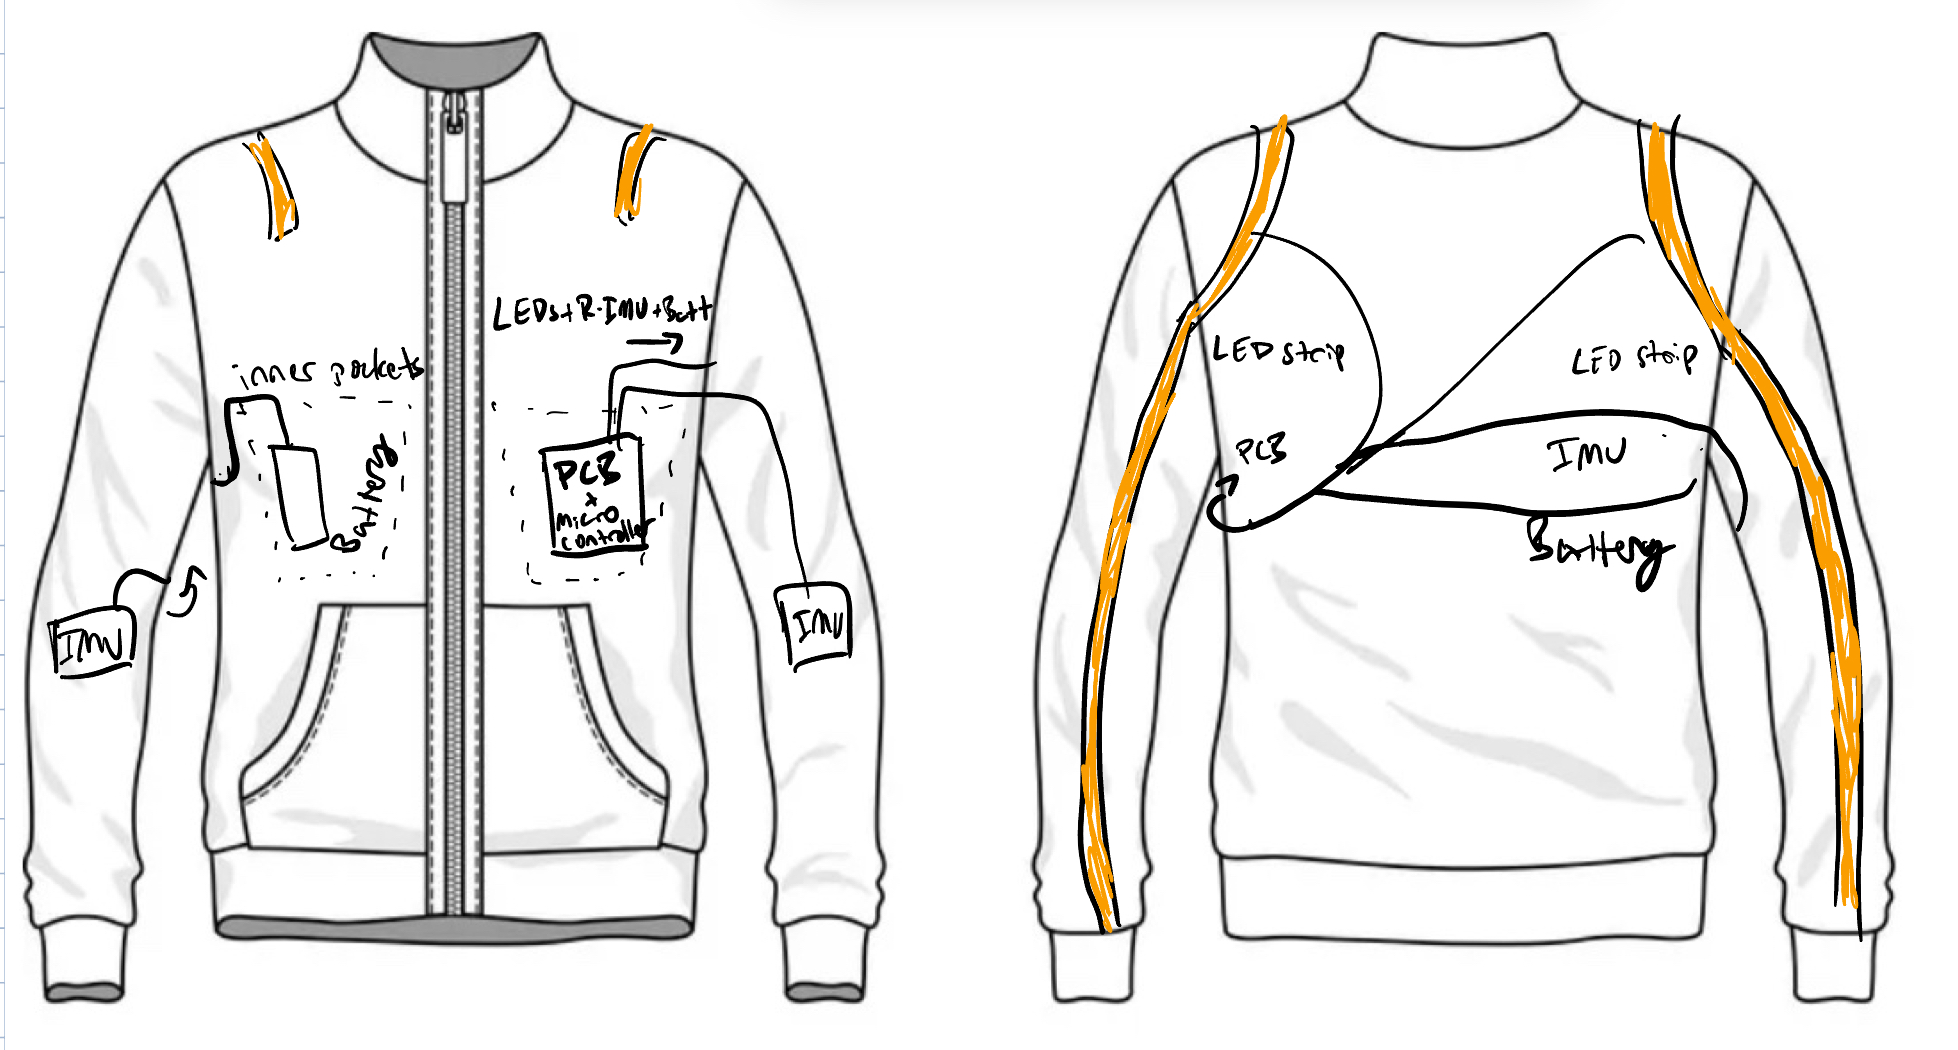
\includegraphics[width=0.8\textwidth]{visual_aid.jpg}
    \caption{Visual Aid mockup of the wearable \cite{VectorStock2024}}
    \label{fig:my_label}
\end{figure}
\subsection{High Level Requirements}
\begin{enumerate}
    \item The device should be able to correctly detect 
    predefined arm gestures (raising right/left arm for 
    turn signals, forearm down for slowing down) with a 
    minimum accuracy of 90\%. 

    \item The device should be able to correctly map the arm 
    gestures into the different indications on the LEDs 
    (turn signal, brake light, hazard).

    \item The turn signals should be visible and easily 
    identifiable from a distance of at least 250 feet in 
    daylight conditions (ex. clear skies at noon) to ensure 
    that they are clearly visible at both day and night. 
\end{enumerate}

\newpage
\section{Design}
\subsection{Block Diagram}
\begin{figure}[ht]
    \centering
    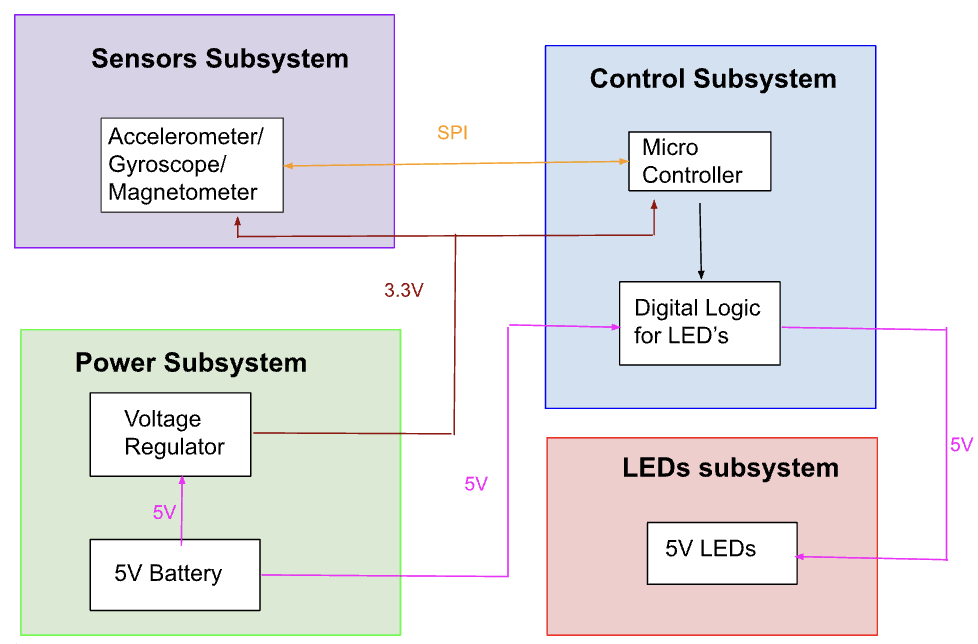
\includegraphics[width=0.8\textwidth]{block_diagram.png}
    \caption{Block Diagram of the system}
    \label{fig:my_label1}
\end{figure}
\subsection{Subsystem Overview}
    \subsubsection{Control Unit:} 
    We will design our PCB and microcontroller to be able to 
    receive data through SPI from the sensors, analyze the data, 
    and display the correct signal on the LEDs. The data will 
    consist of acceleration, rotational, and magnetic orientation
    data from the 9 degrees of freedom (9DoF) IMU. The PCB will 
    contain the microcontroller, power the sensor suite, and 
    contain digital logic to control the LEDs. We will use the 
    ESP32 microcontroller \cite{EspressifESP32} to process the data from the sensors 
    and output the correct signals to the LEDs. 
    \subsubsection{Power Subsystem:} 
	We will use a 5V rechargeable battery (Li-Ion or LiPo) to 
    power the components, 5V for the LEDs, and use a voltage 
    regulator \cite{DiodesIncorporatedAP2112} to power the microcontroller and sensors at 3.3V. 
    We can place the battery in an inner pocket of the wearable,
     making it easy to wire it to all parts. 
    \subsubsection{Sensors Subsystem:} 
    For the sensors, we will use a 3.3V 9dof IMU (accelerometer, 
    gyroscope, magnetometer) \cite{STMicroelectronics2015LSM9DS1} for each arm, and use the combined 
    data from both to determine the nature of the motion. In an 
    accident for example, the acceleration will spike, indicating 
    an accident. To distinguish between the other signals, we will
     use the gyroscope to determine the angle of the gesture. The 
     IMUs will be powered directly by the power subsystem through 
     a voltage regulator to step the voltage down to 3.3V. The 
     sensors will communicate with the ESP32 microcontroller 
     through SPI for data transfer. 
    \subsubsection{LEDs Subsystem:} 
    We will use 5V LED strips placed on the back and arms of the 
    wearable to display the information. The LEDs will be arranged 
    on the back of the arms and over the shoulder from the 
    shoulder blade to the upper chest area (for front visibility). 


\subsection{Subsystem Requirements}

\subsubsection{Control Unit:} 
The control unit should be able to receive SPI data from the 
sensor subsystem and use the ESP32 microcontroller to analyze 
it in order to route the 5V from the battery to power the LEDs. 
To control the LEDs, we will add transistors \cite{MicrochipVN10K} to the PCB. 

\textbf{Requirements:} 
\begin{itemize}
    \item Must be able to communicate with the sensors and LEDs through the PCB
    \item Must be able to properly filter out noise from the sensor data
    \item Must be able to determine the correct movements/accident from the sensor data
\end{itemize}

\subsubsection{Power Subsystem:} 
The Power subsystem should be able to output 5V through the control unit to power the LEDs, as well as output 3.3V to power the Control and Sensors subsystems. 

\textbf{Requirement:} 
\begin{itemize}
    \item Supply sufficient 3.3V-5V power to the 
    other components and subsystems.
\end{itemize}

\subsubsection{Sensors Subsystem:}
The sensor subsystem should contain an IMU (accelerometer, gyroscope, and magnetometer) for each arm, read and controlled by the ESP32 microcontroller via an SPI signal. The data should contain acceleration, rotational, and cardinal direction data and should be filtered properly so as to not miss vital information and not cause false signals. The IMUs will be powered by a 3.3V input via the Power Subsystem.

\textbf{Requirement:}
\begin{itemize}
    \item Must be able to constantly communicate with the 
    ESP32 throughout a power cycle (1 hour). 
\end{itemize}

\subsubsection{LEDs Subsystem:} 
The LED subsystem should be able to turn on the LEDs when powered by a 5V input from the control/power subsystems.

\textbf{Requirement:} 
\begin{itemize}
    \item Must be able to turn on and off when instructed to by the microcontroller.
    \item Must be bright enough for drivers to see at night at a reasonable distance (250 ft).
    \item Must be able to display different colors for turn signals/hazards and braking.
\end{itemize}

\subsection{Tolerance Analysis}
We will be using several components operating at 3.3V and a 5V 
battery that allows recharging. Therefore we need to use a 
voltage regulator to step down the voltage for the sensors 
and the ESP32. 

\noindent ESP32 worst case current draw: 240 mA

\noindent 2 IMUs, current draw for each: 4.6 mA
\begin{align*}
    \text{Input power} &= V_{\text{in}} \times I_{\text{load}} = 5V \times (0.24A + 2 \times 4.6mA) \\
    \text{Output power} &= V_{\text{out}} \times I_{\text{load}} = 3.3V \times (240mA + 2 \times 4.6mA) \\
    \text{Power dissipated} &= P_{\text{in}} - P_{\text{out}} \quad (\text{worst case}) \\
    \text{Temp Rise} &= P_{\text{diss}} \times R_{\text{th}} = 19.9 \, ^{\circ}C \\
    \text{Estimated total temp} &= 25 + 19.9 = 44.9 \, ^{\circ}C
\end{align*}

\noindent The temperature rise is well within the operating range of the voltage regulator, so we can use it for our design.


\noindent Additionally we need to make sure we aren’t 
overloading the battery which can cause overheating. We will 
need to be careful to not cause the battery or the voltage 
regulator to overheat. Overheating would run the risk of 
damaging the rider, as well as affecting the rest of the parts 
negatively.

\noindent LEDs current: \( 2A \) total 

\noindent ESP32 and IMUs: \( 240mA + 2 \times 4.6mA \)
\begin{align*}
\text{Battery Efficiency} &= 90\% \\
P_{\text{total}} &= V \times I = 5(2A + 240mA + 2 \times 4.6mA) = 11.246W \\
P_{\text{loss}} &= \frac{P_{\text{total}}}{\text{Efficiency}} - P_{\text{total}} = 11.246W - 11.246W = 1.25W \\
R_{\text{th}} &= 20 \, ^{\circ}C/W \\
\text{Temp rise} &= P_{\text{loss}} \times R_{\text{th}} = 25 \, ^{\circ}C \\
\text{Total temp} &= 25 + 25 = 50 \, ^{\circ}C
\end{align*}

\section{Ethics and Safety}
\subsection{Ethical Considerations}
The biggest concern as it relates to ethics and safety for 
this project is with regard to the safety of the user and 
those on the road around the user. Under the IEEE code of 
ethics, we are required to prioritize the safety of the 
safety of the public \cite{IEEEethics2024}. If the wearable isn’t user
friendly enough, or restricts any movements, this can lead 
to potentially catastrophic accidents. We can solve this by 
integrating the electronics out of the way of the user, 
such as in the inner pockets of the jacket (for the PCB 
and battery), and providing ample slack in the wires 
throughout. This will allow the user to move more naturally.
Another concern might be the privacy of the user \cite{IEEEethics2024}
because we will be collecting and processing data constantly 
during a ride/commute. We can limit the data collection to 
IMU data, so that nothing personally identifiable is
collected, as well as deleting any data past a certain 
period of time. 




\subsection{Safety Considerations}
The IEEE Code of Ethics mentions that it is important
to “hold paramount the safety, health, and welfare” of 
the public”. \cite{IEEEethics2024}
We have to consider the brightness of the LEDs, 
and if they can be distracting to other drivers and 
pedestrians. Having bright LEDs can be beneficial for 
low light or adverse conditions, but can also be harmful 
if they dazzle other drivers, impairing their vision. 
There aren’t any safety regulatory requirements for 
LEDs for bicycles relating to the brightness of the 
lights, so we make sure we are following the vehicle 
regulations for turn signals. \cite{CFR571_108} 


\newpage
\bibliography{references}


\end{document} 